\chapter{Attacks}
\label{chapter:attacks}

  In recent work He et al. \cite{DBLP:journals/corr/abs-2005-02131} proposed the first link stealing attacks on graph neural networks.
  They focused on stealing links of the graph, that was used for training the given target model.
  Like described in Section 3.3.1 this is an attack on transductive trained graph neural networks.
  In our work, we want to show, that it is possible for an adversary to steal links from any graphs, given black-box access to an inductive trained target graph neural network model.

  \section{Adversary's Goal}

    Let $f_t$ be the target graph neural network model, trained to perform some machine learning task.
    Let $G_s = (V_s, E_s)$ be a graph with $|V_s|$ nodes and $|E_s|$ edges. 
    We assume, that some of $G_s$'s links/edges are missing.
    The goal of an adversary $A$ is, to infer whether two nodes $i,j \in V_s$ are connected to each other or not.
    More precisely, whether the link $(i,j)$ between the nodes $i$ and $j$ is missing, or does not exist.
  
  \section{Intuition}

    Since $A$ has black box access to its target model, it will use the posterior output of $f_t$, to make its classification.
    To do so, $A$ queries $f_t$ on two nodes $i,j \in V_s$, from which it want's to know whether they are linked or not.
    For both nodes $f_t$ will return a posterior: $post_i = f_t(G_s, i)$ and $post_j = f_t(G_s, j)$.
    $A$ can be trained on how the two posteriors "look like", when $i$ and $j$ originally have been connected and the edge is missing in $G_s$ or how they look like when there is no edge to recover.


  \section{Threat Model}

    For any of our attacks, we assume, \emph{Black-Box Access} (Query Access) to the target graph neural network model $f_t$, that was trained on a graph dataset $D_{f_t}$.
    We consider $f_A$ another graph neural network model, which was trained by the adversary using a graph dataset $D_{f_A}$.
    The adversary $A$ was trained on a dataset $D_A$ to perform link stealing attacks.
    We denote $G_A = (V_A, E_A)$ as graph used by the adversary querying $f_A$ to sample $D_A$.
    We assume, that in any attack $D_{f_t}$ and $G_s$ are from the same dataset distribution, as well as $D_{f_A}$ and $G_A$ share the same one.
    However, $D_{f_A}$ must not be from the same dataset distribution as $D_{f_t}$.
    For \emph{Attack 1} and \emph{Attack 2} we consider $f_t = f_A$, which implies $D_{f_t} = D_{f_A}$. 
    Table \refeq{table:notations} can be used to look up notation descriptions.

    \begin{figure}[h!]
      \begin{tikzpicture}
        % \draw[step=1cm,gray,very thin] (-8,-5) grid (8,4);
        \draw (-0.65 ,3.8) -- (-0.65,-2.8);
        \draw (-8,4) -- (6.7,4);
        \draw (-8,-3) -- (6.7,-3);
        
        % SDD
        \draw (-4.65,-2.5) node (a) {\emph{Attack 1-2}};
        \draw (-4.65,1) ellipse (3cm and 1.5cm);
        \draw (-7.65,0) node (a) {$d$};
        \draw (-6.65,1) node (a) {$D_{f_t}$};
        \draw (-4.65,1) node (a) {$G_A$};
        \draw (-2.65,1) node (a) {$G_s$};
        
        % DDD
        \draw (3.35,-2.5) node (a) {\emph{Attack 3}};
        \draw (3.35,2.5) ellipse (3cm and 1cm);
        \draw (0.35,2) node (a) {$d_1$};
        \draw (2.35,2.5) node (a) {$D_{f_t}$};
        \draw (4.35,2.5) node (a) {$G_s$};
        \draw (3.35,-0.5) ellipse (3cm and 1cm);
        \draw (0.35,-1) node (a) {$d_2$};
        \draw (2.35,-0.5) node (a) {$D_{f_A}$};
        \draw (4.35,-0.5) node (a) {$G_A$};

      \end{tikzpicture}
      \caption{Dataset Distributions for Link Stealing Attacks}
      \label{figure:dataset-distribution}
    \end{figure}

    

  \section{Attack Methodology}

    % TODO
    Let $f_t$ be the target graph neural network model and $G_s = (V_s, E_s)$ a graph with $|V_s|$ nodes and $|E_s|$ edges.
    We assume that $E_s$ is not complete. 
    More precisely, there exists an edge $(i,j)$ between the nodes $i,j \in V_s$, but $(i,j) \not\in E_s$.
    The adversary $A$ queries $f_t$ on both nodes $i$ and $j$, obtaining $post_i = f_t(G_s, i)$ and $post_j = f_t(G_s, j)$.

    \subsection{Attack 1}
      In \emph{Attack 1} we consider $G_A$ and $D_{f_t}$ from the same dataset distribution and denote $f_t = f_A$.
      Meaning, that $A$ samples its training dataset $D_A$ by querying $f_t$.
      That can be done, because $|post_u| = |f_t(G_A,u)|$ (training phase) and $|post_v| = |f_t(G_s,v)|$ (attack phase), with $u \in V_A$ and $v \in V_s$, have the same dimension.
      Based on this assumption, $A$ can directly be trained on the posteriors generated by $f_t$.
      Therefore we concatenate $post_i$ and $post_j$ obtaining the input $post_{ij} = cat(post_i, post_j)$, with $cat(A,B) = [a_0,...,a_n,b_0,...,b_n]$, where $A = [a_0,...,a_n]$ and $B = [b_0,...,b_n]$. 
      Given $post_{ij}$, $A$ can infer, whether $i$ and $j$ have been connected and the edge is missing in $G_s$ or not.

      \vspace{0.48cm}
      \begin{figure}[h!]
        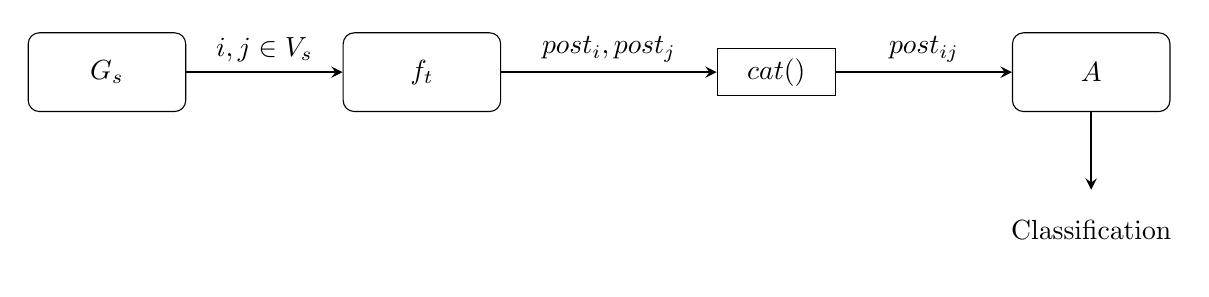
\begin{tikzpicture}
          
          % Definitions
          \tikzstyle{A} = [rectangle, rounded corners, minimum width=2cm, minimum height=1cm,text centered, draw=black]
          \tikzstyle{f_t} = [rectangle, rounded corners, minimum width=2cm, minimum height=1cm,text centered, draw=black]
          \tikzstyle{G_s} = [rectangle, rounded corners,minimum width=2cm, minimum height=1cm, text centered, draw=black]
          \tikzstyle{sample} = [rectangle, minimum width=1.5cm, minimum height=0.6cm, text centered, draw=black]
          \tikzstyle{dec} = [rectangle, minimum width=2cm, minimum height=1cm, text centered]
          \tikzstyle{arrow} = [thick,->,>=stealth]

          \node (G_s) [G_s] {$G_s$};
          \node (f_t) [f_t, right of=G_s, xshift=3cm] {$f_t$};
          \node (sample) [sample, right of=f_t, xshift=3.5cm] {$cat()$};
          \node (A) [A, right of=sample, xshift=3cm] {$A$};
          \node (dec) [dec, below of=A, yshift=-1cm] {Classification};

          \draw [arrow] (G_s) -- node[anchor=south] {$i,j \in V_s$} (f_t);
          \draw [arrow] (f_t) -- node[anchor=south] {$post_i, post_j$} (sample);
          \draw [arrow] (sample) -- node[anchor=south] {$post_{ij}$} (A);
          \draw [arrow] (A) -- (dec);

        \end{tikzpicture}
        \caption{Flow Chart - Attack 1}
        \label{figure:flow-chart-attack-1}
      \end{figure}

    \subsection{Attack 3}
      In \emph{Attack 3} we consider $G_A$ and $D_{f_t}$ from different dataset distributions.
      So the adversary trains another graph neural network model $f_A$ with a dataset $D_{f_A}$.
      Since $f_t$ and $f_A$ are trained on different dataset distributions, we must assume that they have different parameters like feature amount or number of classes. 
      Meaning, that it is not possible anymore, to train the adversary directly on the posterior output of $f_t$, since $|post_u| = |f_A(G_A,u)|$ (training phase) and $|post_v| = |f_t(G_s,v)|$ (attack phase), with $u \in V_A$ and $v \in V_s$, have different dimensions.
      Based on this assumption, we need to sample the input for $A$, by creating features based on the posteriors, instead of using them directly.
      As features we use eight common distance metrics, to measure the distance between $post_i$ and $post_j$.
      We have in total experimented with Cosine distance, Euclidean distance, Correlation distance, Chebyshev distance, Braycurtis distance, Canberra distance, Manhattan distance, and Square-euclidean distance.
      The formal definition of each distance metrics is listed in table \refeq{table:distance}.
      So we construct the input $dist_{ij}$ for $A$ as follows: $dist_{ij} = dist(post_i, post_j)$, where $dist(post_i, post_j) = [Cosine(post_i,post_j), ..., Sqeuclidean(post_i,post_j)]$.
      Given $dist_{ij}$, $A$ now can infer, whether $i$ and $j$ have been connected and the edge is missing in $G_s$ or not.

      \vspace{0.48cm}
      \begin{figure}[h!]
        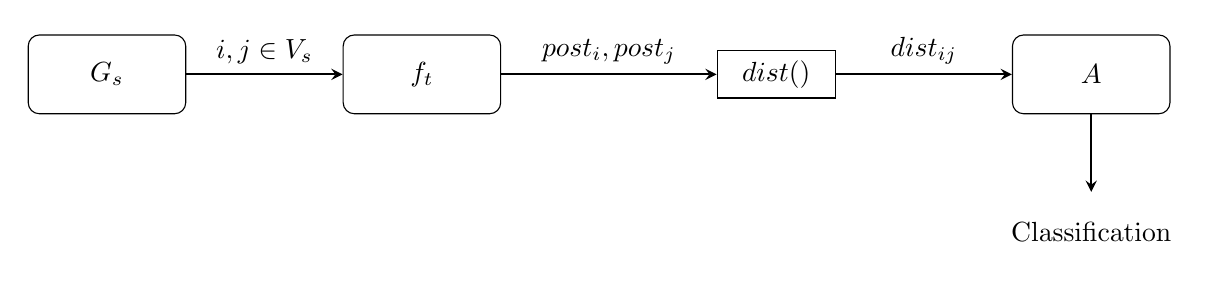
\begin{tikzpicture}
          
          % Definitions
          \tikzstyle{A} = [rectangle, rounded corners, minimum width=2cm, minimum height=1cm,text centered, draw=black]
          \tikzstyle{f_t} = [rectangle, rounded corners, minimum width=2cm, minimum height=1cm,text centered, draw=black]
          \tikzstyle{G_s} = [rectangle, rounded corners,minimum width=2cm, minimum height=1cm, text centered, draw=black]
          \tikzstyle{sample} = [rectangle, minimum width=1.5cm, minimum height=0.6cm, text centered, draw=black]
          \tikzstyle{dec} = [rectangle, minimum width=2cm, minimum height=1cm, text centered]
          \tikzstyle{arrow} = [thick,->,>=stealth]

          \node (G_s) [G_s] {$G_s$};
          \node (f_t) [f_t, right of=G_s, xshift=3cm] {$f_t$};
          \node (sample) [sample, right of=f_t, xshift=3.5cm] {$dist()$};
          \node (A) [A, right of=sample, xshift=3cm] {$A$};
          \node (dec) [dec, below of=A, yshift=-1cm] {Classification};

          \draw [arrow] (G_s) -- node[anchor=south] {$i,j \in V_s$} (f_t);
          \draw [arrow] (f_t) -- node[anchor=south] {$post_i, post_j$} (sample);
          \draw [arrow] (sample) -- node[anchor=south] {$dist_{ij}$} (A);
          \draw [arrow] (A) -- (dec);

        \end{tikzpicture}
        \caption{Flow Chart - Attack 3}
        \label{figure:flow-chart-attack-3}
      \end{figure}

    \newpage
    \subsection{Attack 2}
      In \emph{Attack 2} we consider $G_A$ and $D_{f_t}$ from the same dataset distribution and denote $f_t = f_A$ like it was done in \emph{Attack 1}.
      However, for better comparison of the impact of the dataset distribution, we sample the input for $A$, like it was done in \emph{Attack 3}.

      \vspace{0.48cm}
      \begin{figure}[h!]
        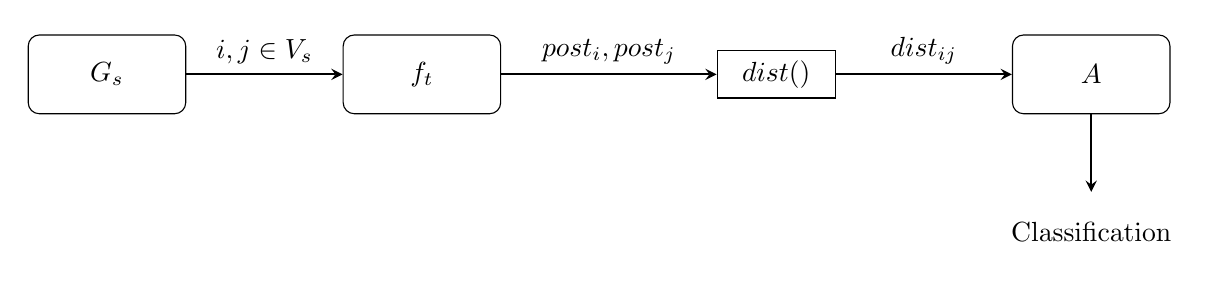
\begin{tikzpicture}
          
          % Definitions
          \tikzstyle{A} = [rectangle, rounded corners, minimum width=2cm, minimum height=1cm,text centered, draw=black]
          \tikzstyle{f_t} = [rectangle, rounded corners, minimum width=2cm, minimum height=1cm,text centered, draw=black]
          \tikzstyle{G_s} = [rectangle, rounded corners,minimum width=2cm, minimum height=1cm, text centered, draw=black]
          \tikzstyle{sample} = [rectangle, minimum width=1.5cm, minimum height=0.6cm, text centered, draw=black]
          \tikzstyle{dec} = [rectangle, minimum width=2cm, minimum height=1cm, text centered]
          \tikzstyle{arrow} = [thick,->,>=stealth]

          \node (G_s) [G_s] {$G_s$};
          \node (f_t) [f_t, right of=G_s, xshift=3cm] {$f_t$};
          \node (sample) [sample, right of=f_t, xshift=3.5cm] {$dist()$};
          \node (A) [A, right of=sample, xshift=3cm] {$A$};
          \node (dec) [dec, below of=A, yshift=-1cm] {Classification};

          \draw [arrow] (G_s) -- node[anchor=south] {$i,j \in V_s$} (f_t);
          \draw [arrow] (f_t) -- node[anchor=south] {$post_i, post_j$} (sample);
          \draw [arrow] (sample) -- node[anchor=south] {$dist_{ij}$} (A);
          \draw [arrow] (A) -- (dec);

        \end{tikzpicture}
        \caption{Flow Chart - Attack 2}
        \label{figure:flow-chart-attack-2}
      \end{figure}

    Furthermore, for each Attack we assume different amounts of edges given in $G_A$. 
    The percentage of known edges is denoted as $\alpha$ and has an impact on the prediction (posteriors) of $f_t$ and $f_A$.
    Therefor we construct new adversary graphs: $G_A^\alpha = (V_A^\alpha, E_A^\alpha)$ with $|E_A^\alpha| = \alpha * |E_A|$ and $V_A^\alpha = V_A$. 
    As different stages we define $\alpha = 0.0, 0.2, 0.4, 0.6, 0.8$. 
    The first case, $\alpha = 0.0$ represents an adversary graph $G_A^{0.0} = (V_A^{0.0}, E_A^{0.0})$ without any edges / no knowledge of the relationship between the nodes.
    $\alpha = 0.8$ leads to an adversary graph $G_A^{0.8} = (V_A^{0.8}, E_A^{0.8})$ with almost every edge considered to be known.

    The following table shows all three attacks with the dataset distribution, the input for the adversary $A$ and the feature amount of $A$.

    \vspace{0.48cm}
    \begin{table}[!h]
      \centering
      \footnotesize
      \begin{tabular}{l|l|l|l}
        \toprule
        Attacks & Dataset Distribution & Input for $A$ & $A$'s Feature Amount\\
        \midrule
        Attack 1 & Same & $inp_{ij} = cat(post_i, post_j)$ & $|inp_{ij}| = |post_i| + |post_j| = 2 * |post_i|$ \\
        Attack 2 & Same & $inp_{ij} = dist(post_i, post_j)$ & $|inp_{ij}| = 8$ \\
        Attack 3 & Different & $inp_{ij} = dist(post_i, post_j)$ & $|inp_{ij}| = 8$ \\
        \bottomrule
      \end{tabular}
      \caption{Attack Methodology}
      \label{table:attack-methodology}
    \end{table}

    

    
  